\documentclass[14pt]{article}
%General Packages
\usepackage{multicol, enumerate, enumitem, hyperref, color, soul, setspace, parskip, fancyhdr}

%Math Packages
\usepackage{amssymb, amsthm, amsmath, bbm, latexsym, units, mathtools}

%All math in Display Style
\everymath{\displaystyle}

% Packages with additional options
%\usepackage[T1]{fontenc}
\usepackage[headsep=0.5cm,headheight=0cm, left=1 in,right= 1 in,top= 1 in,bottom= 1 in]{geometry}
\usepackage[usenames,dvipsnames]{xcolor}

% SageTeX
\usepackage{sagetex}

% Package to use the command below to create lines between items
\usepackage{dashrule}
\newcommand{\litem}[1]{\item#1\hspace*{-1cm}\rule{\textwidth}{0.4pt}}

\pagestyle{fancy}
\lhead{Module\,6\,-\,Polynomial\,Functions}
\chead{}
\rhead{Progress Exam 3}
\lfoot{Summer\,C\,2020}
\cfoot{}
\rfoot{Version B}

\begin{document}
\pagestyle{fancy}

\begin{sagesilent}
load("../Code/generalPurposeMethods.sage")
load("../Code/keyGeneration.sage")
keyFileName = "Module6"
version = "B"
\end{sagesilent}

\begin{enumerate}
\setcounter{enumi}{25}


\begin{sagesilent}
moduleNumber=6
problemNumber=26
load("../Code/polynomial/constructPolyComplex.sage")
\end{sagesilent}

\litem{	\sage{displayStem}

	\[ \sage{displayZero1} \text{ and } \sage{displayZero2} \]

	\begin{enumerate}[label=\Alph*.]
		\item \( \sage{choices[0]} \)
		\item \( \sage{choices[1]} \)
		\item \( \sage{choices[2]} \)
		\item \( \sage{choices[3]} \)
		\item \( \sage{choices[4]} \)
	\end{enumerate}
}

\begin{sagesilent}
moduleNumber=6
problemNumber=27
load("../Code/polynomial/polyZeroBehavior.sage")
\end{sagesilent}

\litem{ \sage{displayStem}

	\[ f(x) = \sage{displayPolynomial} \]

\begin{multicols}{4}
	\begin{enumerate}[label=\Alph*.]
		\item \begin{center} 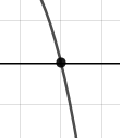
\includegraphics[width=.2\textwidth]{../Figures/zeroBehaviorNegativeOddB}\end{center}
    \columnbreak
		\item \begin{center} 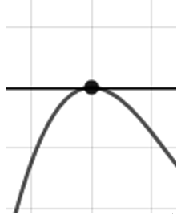
\includegraphics[width=.2\textwidth]{../Figures/zeroBehaviorNegativeEvenB}\end{center}
    \columnbreak
		\item \begin{center} 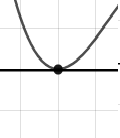
\includegraphics[width=.2\textwidth]{../Figures/zeroBehaviorPositiveEvenB}\end{center}
    \columnbreak
		\item \begin{center} 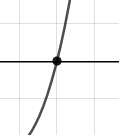
\includegraphics[width=.2\textwidth]{../Figures/zeroBehaviorPositiveOddB}\end{center}
	\end{enumerate}
\end{multicols}
}

\begin{sagesilent}
moduleNumber=6
problemNumber=28
load("../Code/polynomial/polyGraphToFunction.sage")
\end{sagesilent}

\litem{ \sage{displayStem}

	\begin{center}
	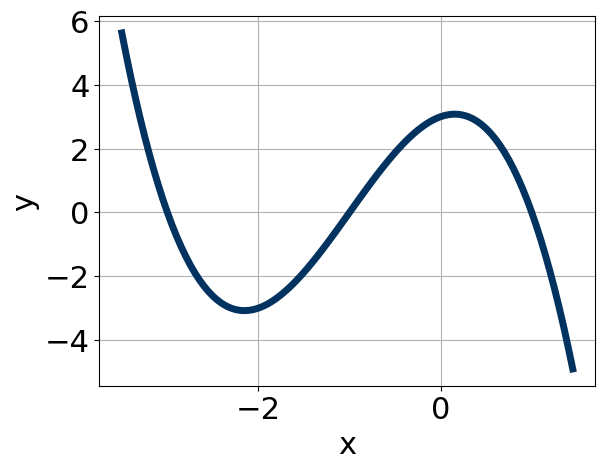
\includegraphics[width = 0.3\textwidth]{../Figures/polyGraphToFunctionB.png}
	\end{center}

	\begin{enumerate}[label=\Alph*.]
		\item \( \sage{choices[0]} \)
		\item \( \sage{choices[1]} \)
		\item \( \sage{choices[2]} \)
		\item \( \sage{choices[3]} \)
		\item \( \sage{choices[4]} \)
	\end{enumerate}
}

\begin{sagesilent}
moduleNumber=6
problemNumber=29
load("../Code/polynomial/polyEndBehavior.sage")
\end{sagesilent}

\litem{ \sage{displayStem}

	\[ f(x) = \sage{displayPolynomial} \]

\begin{multicols}{4}
	\begin{enumerate}[label=\Alph*.]
		\item \begin{center} 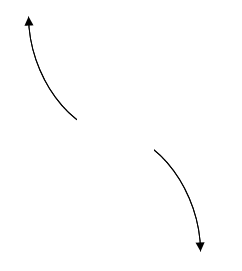
\includegraphics[width=.2\textwidth]{../Figures/endBehaviorNegativeOddB} \end{center}
    \columnbreak
		\item \begin{center} 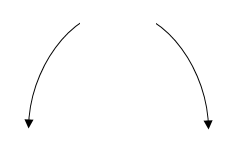
\includegraphics[width=.2\textwidth]{../Figures/endBehaviorNegativeEvenB}\end{center}
    \columnbreak
		\item \begin{center} 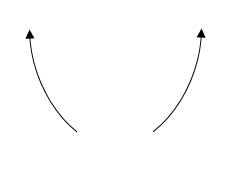
\includegraphics[width=.2\textwidth]{../Figures/endBehaviorPositiveEvenB}\end{center}
    \columnbreak
		\item \begin{center} 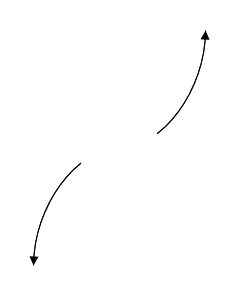
\includegraphics[width=.2\textwidth]{../Figures/endBehaviorPositiveOddB}\end{center}
	\end{enumerate}
\end{multicols}
}

\begin{sagesilent}
moduleNumber=6
problemNumber=30
load("../Code/polynomial/constructPolyRationals.sage")
\end{sagesilent}

\litem{ \sage{displayStem}

	\[ \sage{displayZero1}, \sage{displayZero2}, \sage{displayZero3} \]

	\begin{enumerate}[label=\Alph*.]
		\item \( \sage{choices[0]} \)
		\item \( \sage{choices[1]} \)
		\item \( \sage{choices[2]} \)
		\item \( \sage{choices[3]} \)
		\item \( \sage{choices[4]} \)
	\end{enumerate}
}

\end{enumerate}

\end{document}

